\documentclass[aspectratio=1610]{beamer}
\usepackage[T1]{fontenc}
\usetheme{wildcat}


\title{Wildcat Beamer Theme}
\date{January 2024}
\author{Aaron Wolf (Northwestern University)}

% You change the titlegraphic to whatever you want, or comment it out to remove it.
\titlegraphic{\includegraphics[scale=0.25]{logo-northwestern.pdf}}

% % You can directly change the colors using the following macros.
% % You must redefine colors AFTER the theme is loaded.
% % For example, these provide shades of Yale Blue (#00356b)
% \definecolor{wcprimary}{RGB}{0,53,107}      % Main color
% \definecolor{wcprimary140}{RGB}{0, 34, 70}
% \definecolor{wcprimary130}{RGB}{0, 40, 80}
% \definecolor{wcprimary120}{RGB}{0, 45, 91}
% \definecolor{wcprimary110}{RGB}{0, 50, 102}
% \definecolor{wcprimary40}{RGB}{153, 174, 196}
% \definecolor{wcprimary30}{RGB}{179, 194, 211}
% \definecolor{wcprimary20}{RGB}{204, 215, 225}
% \definecolor{wcprimary10}{RGB}{230, 235, 240}

% % Now for the alerted orange (#bd5319) and example green (#5f712d)
% \definecolor{wcalerted}{RGB}{189,83,25}
% \definecolor{wcexample}{RGB}{95,113,45}

% % If you want to change the slide background color, 
% % you can use the following command:
%\setbeamercolor{background canvas}{bg=nupurple10!30}

% % Turn off section slides
% \AtBeginSection{}

% Change the font theme
%\usefonttheme{wildcat-overleaf}

% Change the bg pattern manually: Simple Single Color
% \renewcommand{\bgpattern}{
%     \draw[color=wcprimary,fill=wcprimary] (0,0) rectangle (\paperwidth,\paperheight);
% }



\begin{document}

\begin{frame}
\titlepage
\end{frame}

% \begin{frame}{Table of Contents}
%     \tableofcontents
% \end{frame}

\begin{frame}{Introduction}
    The Wildcat theme is a Beamer theme for Northwestern University, but which can be modified easily with different colors, fonts, and even background patterns. 
    \\ ~ \\
    The theme is inspired by the \href{https://github.com/matze/mtheme}{Metropolis theme} by Matthias Vogelgesang. It incorporates the Northwestern University facet design pattern, but otherwise has a clean, simple look, and relatively few bells and whistles. It is licensed under the GNU GENERAL PUBLIC LICENSE.
\end{frame}

\begin{frame}
    \frametitle{Colors}
    The theme has a few Northwestern-specific colors defined, which you can use in your slides. These are:
    \begin{columns}
    \column{0.3\textwidth}
    \begin{itemize}
        \item[$\textcolor{nupurple}{\bullet}$] \textcolor{nupurple}{nupurple} 
        \item[$\textcolor{nupurple90}{\bullet}$] \textcolor{nupurple90}{nupurple90} 
        \item[$\textcolor{nupurple80}{\bullet}$] \textcolor{nupurple80}{nupurple80}
        \item[$\textcolor{nupurple70}{\bullet}$] \textcolor{nupurple70}{nupurple70}
        \item[$\textcolor{nupurple60}{\bullet}$] \textcolor{nupurple60}{nupurple60}
        \item[$\textcolor{nupurple50}{\bullet}$] \textcolor{nupurple50}{nupurple50}
        \item[$\textcolor{nupurple40}{\bullet}$] \textcolor{nupurple40}{nupurple40}
        \item[$\textcolor{nupurple30}{\bullet}$] \textcolor{nupurple30}{nupurple30}
        \item[$\textcolor{nupurple20}{\bullet}$] \textcolor{nupurple20}{nupurple20}
        \item[$\textcolor{nupurple10}{\bullet}$] \textcolor{nupurple10}{nupurple10}
    \end{itemize}
    \column{0.3\textwidth}
    \begin{itemize}
        \item[$\textcolor{nupurple160}{\bullet}$] \textcolor{nupurple160}{nupurple160}
        \item[$\textcolor{nupurple150}{\bullet}$] \textcolor{nupurple150}{nupurple150}
        \item[$\textcolor{nupurple140}{\bullet}$] \textcolor{nupurple140}{nupurple140}
        \item[$\textcolor{nupurple130}{\bullet}$] \textcolor{nupurple130}{nupurple130}
        \item[$\textcolor{nupurple120}{\bullet}$] \textcolor{nupurple120}{nupurple120}
        \item[$\textcolor{nupurple110}{\bullet}$] \textcolor{nupurple110}{nupurple110}
        \item[$\textcolor{nurichblack}{\bullet}$] \textcolor{nurichblack}{nurichblack}
        \item[$\textcolor{nubrightgreen}{\bullet}$] \textcolor{nubrightgreen}{nubrightgreen}
        \item[$\textcolor{nubrightteal}{\bullet}$] \textcolor{nubrightteal}{nubrightteal}
        \item[$\textcolor{nubrightblue}{\bullet}$] \textcolor{nubrightblue}{nubrightblue}
    \end{itemize}
    \column{0.3\textwidth}
    \begin{itemize}
        \item[$\textcolor{nubrightyellow}{\bullet}$] \textcolor{nubrightyellow}{nubrightyellow}
        \item[$\textcolor{nubrightorange}{\bullet}$] \textcolor{nubrightorange}{nubrightorange}
        \item[$\textcolor{nubrightred}{\bullet}$] \textcolor{nubrightred}{nubrightred}
        \item[$\textcolor{nudarkgreen}{\bullet}$] \textcolor{nudarkgreen}{nudarkgreen}
        \item[$\textcolor{nudarkteal}{\bullet}$] \textcolor{nudarkteal}{nudarkteal}
        \item[$\textcolor{nudarkblue}{\bullet}$] \textcolor{nudarkblue}{nudarkblue}
        \item[$\textcolor{nudarkyellow}{\bullet}$] \textcolor{nudarkyellow}{nudarkyellow}
        \item[$\textcolor{nudarkorange}{\bullet}$] \textcolor{nudarkorange}{nudarkorange}
        \item[$\textcolor{nudarkred}{\bullet}$] \textcolor{nudarkred}{nudarkred}
    \end{itemize}
    \end{columns}
\end{frame}

\begin{frame}{Modifying Main Colors (I)}
    You can change the main colors of the theme by redefining the following colors in your preamble. You can use any color you want, but the theme is designed to work best with shades of the Northwestern purple.
    \begin{itemize}
        \item \texttt{wcprimary} (main color)
        \item \texttt{wcprimary10} (main color, 10\% shade) through \texttt{wcprimary40} (main color, 40\% shade)
        \item \texttt{wcprimary110} (main color, 110\% shade) through \texttt{wcprimary160} (main color, 160\% shade)
        \item \texttt{wcalerted} (alert color)
        \item \texttt{wcexample} (example color)
    \end{itemize}
   The shades of wcprimary are used for the background of facets. There are wcprimary10, wcprimary20, ..., wcprimary160, but only 10-40 and 110-140 are used.
\end{frame}

\begin{frame}[fragile]
    \frametitle{Modifying Main Colors (II)}
    For example, to modify the main color to be a shade of blue, you could use the following code in your preamble (after loading the theme):
    \begin{verbatim}
        \definecolor{wcprimary}{RGB}{0,53,107}
        \definecolor{wcprimary140}{RGB}{0, 34, 70}
        \definecolor{wcprimary130}{RGB}{0, 40, 80}
        \definecolor{wcprimary120}{RGB}{0, 45, 91}
        \definecolor{wcprimary110}{RGB}{0, 50, 102}
        \definecolor{wcprimary40}{RGB}{153, 174, 196}
        \definecolor{wcprimary30}{RGB}{179, 194, 211}
        \definecolor{wcprimary20}{RGB}{204, 215, 225}
        \definecolor{wcprimary10}{RGB}{230, 235, 240}
    \end{verbatim}
    This sets the main color to Yale Blue, and all the shades used in the facet pattern. The preambles of the example slides in this document show how to modify the colors.
\end{frame}

\begin{frame}[fragile]
    \frametitle{Using Colors in Graphs}
    %You can use the colors in your graphs in Python, R, and Stata using the following commands:
    \begin{tblock}{Python Code}
        \footnotesize
        \begin{verbatim}
import matplotlib.pyplot as plt
import pandas as pd
plt.style.use('ggplot')
# Create colors
wcprimary = (78/255,42/255,132/255)
df = pd.read_stata("source/graphs/auto.dta")
plt.scatter(df["weight"], df["mpg"], color=wcprimary)
plt.xlabel("Weight")
plt.ylabel("MPG")
plt.savefig("source/graphs/plot-python.pdf")
plt.show()
        \end{verbatim}
    \end{tblock}
\end{frame}

\begin{frame}[fragile]
    \frametitle{Using Colors in Graphs}
    \begin{figure}
        \centering
        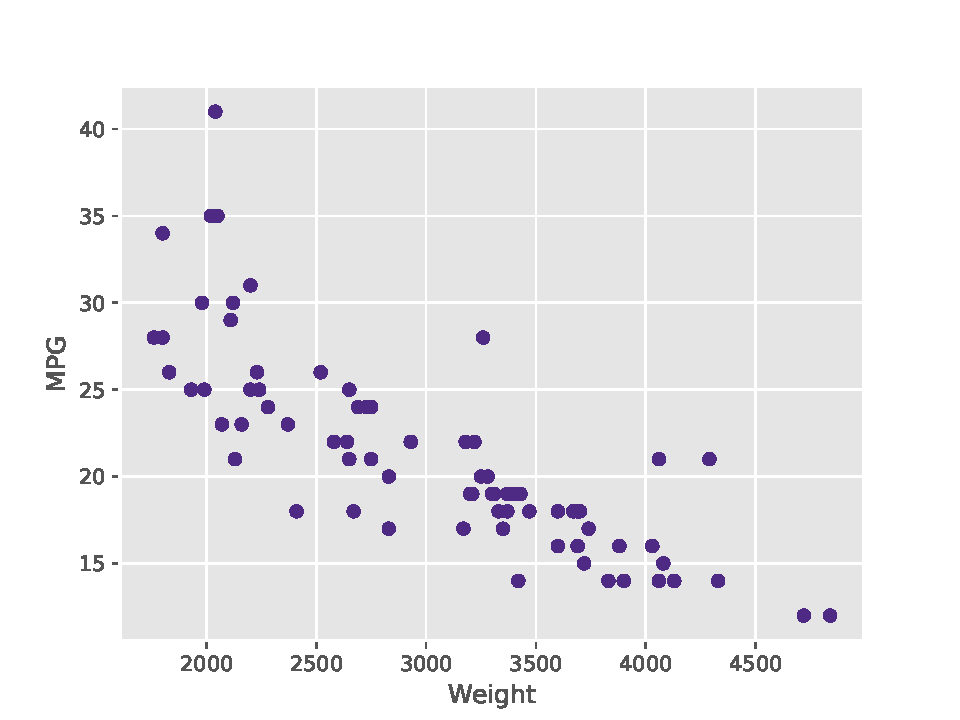
\includegraphics[width=0.7\textwidth]{graphs/plot-python.pdf}
        \caption{Python Graph Example}
        \label{fig:graph-python}
    \end{figure}
\end{frame}

\begin{frame}[fragile]
    \frametitle{Using Colors in Graphs}
    \begin{tblock}{R Code}
        \footnotesize
        \begin{verbatim}
library(ggplot2)
library(haven)
# Load data
df <- read_dta("source/graphs/auto.dta")
# Define custom RGB colors
wcprimary <- rgb(78/255, 42/255, 132/255)

# Plot mpg against weight, with marker color wcprimary
plot <- ggplot(df, aes(x = weight, y = mpg)) +
    geom_point(color = wcprimary) +
    labs(x = "Weight", y = "MPG")

# Save the plot to a file with a specific size
ggsave("source/graphs/plot-R.pdf", plot, width = 8, height = 5)
        \end{verbatim}
    \end{tblock}
\end{frame}



\begin{frame}[fragile]
    \frametitle{Using Colors in Graphs}
    \begin{figure}
        \centering
        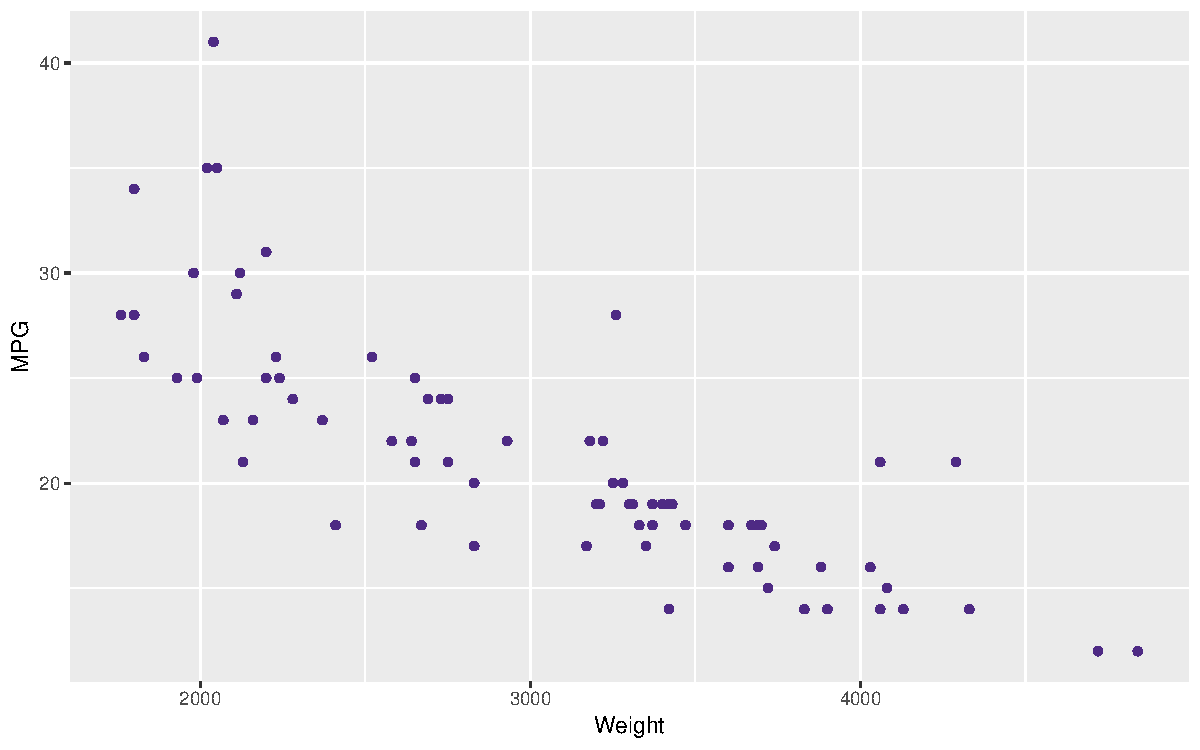
\includegraphics[width=0.8\textwidth]{graphs/plot-R.pdf}
        \caption{R Graph Example}
        \label{fig:graph-R}
    \end{figure}
\end{frame}

\begin{frame}[fragile]
    \frametitle{Using Colors in Graphs}
    \begin{tblock}{Stata Code}
        \footnotesize
        \begin{verbatim}
*ssc install schemepack, replace
sysuse auto, clear
local wcprimary "78 42 132"

twoway (scatter mpg weight, mcolor("`wcprimary'")), ///
        scheme(gg_tableau)
        
graph export "plot-stata.pdf", replace
        \end{verbatim}
    \end{tblock}
\end{frame}

\begin{frame}[fragile]
    \frametitle{Using Colors in Graphs}
    \begin{figure}
        \centering
        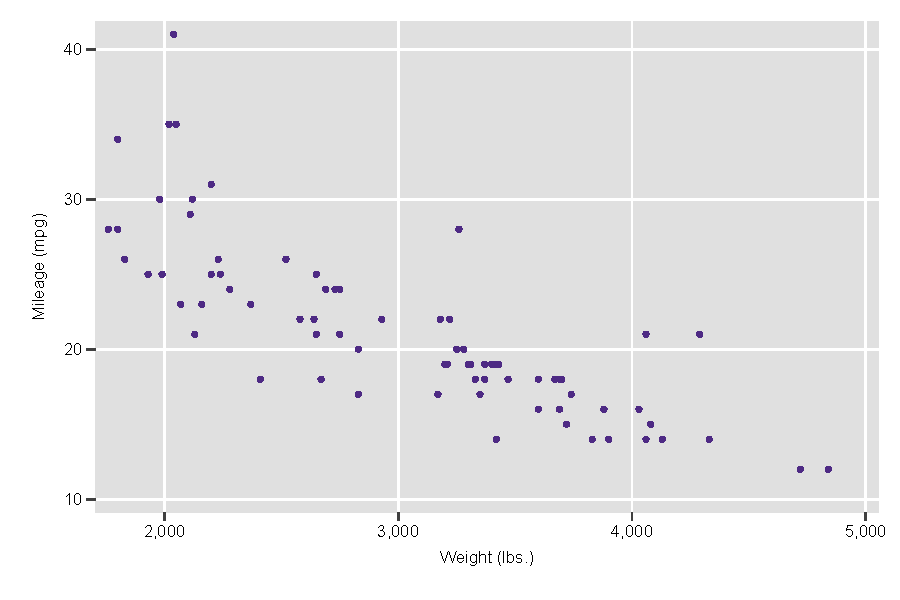
\includegraphics[width=0.7\textwidth]{graphs/plot-stata.pdf}
        \caption{Stata Graph Example}
        \label{fig:graph-stata}
    \end{figure}
\end{frame}


\begin{frame}{Facet Blocks (tcolorbox)}
    You can use tcolorbox style blocks with the facet pattern instead of the default beamer blocks. You can create this with a \texttt{\textbackslash begin\{tblock\}} environment. You can also use \texttt{talert} and \texttt{texample} for alert and example blocks, respectively.
    \begin{tblock}{T Block Title}
        This is a tcolorbox style block.
    \end{tblock}
    \begin{talert}{T Alert Title}
        This is a tcolorbox style alert block.
    \end{talert}
    \begin{texample}{T Example Title}
        This is a tcolorbox style example block.
    \end{texample}
\end{frame}

\begin{frame}[fragile]{Custom Color Facet Blocks}
    There is also a special block called \texttt{tfacetbox} which allows you to specify the color. This only works with non-primary (not red, green, or blue) colors, as you can't shade those easily.
    \begin{tfacetbox}[nudarkyellow]{Custom Facet Block Title}
        This is a tfacetbox block. It can be created with the following code:
        \begin{verbatim}
\begin{tfacetbox}[nudarkyellow]{Custom Facet Block Title}
    This is a tfacetbox block...
\end{tfacetbox}
        \end{verbatim}
    \end{tfacetbox}
\end{frame}

\begin{frame}
    \frametitle{Box Examples (Default)}
    You can also just use the Beamer default blocks in the usual way. The default is non-rounded corners, non-shaded.
    \begin{block}{Main Block}
    This is an example block
    \end{block}
    \begin{alertblock}{Alert Box}
    This is an alert box
    \end{alertblock}
    \begin{exampleblock}{Example Box}
        This is an example box
    \end{exampleblock}
    \end{frame}

\begin{frame}{Font Style: Default}
    The theme uses the official Northwestern fonts, which are Campton (for titles) and Akkurat Pro (for copy). These are not free fonts, so you will need to purchase (and install) them if you want to use them.
    \\ ~ \\
    The wildcat theme uses the OTF files directly, so as long as you have the OTFs in a similar relative directory as the demo files, it should work (this includes on Overleaf). If you have installed them, you can look at the \texttt{\textbackslash beamerfontthemewildcat-installed.sty} file to see how to use the installed fonts.
    \\ ~ \\
    Note: You need to us XeLaTeX or LuaLaTeX to compile in order to use custom fonts. If you use PDFLaTeX, you will get an error.
\end{frame}

\begin{frame}{Font Style: Overleaf \& Local}
    There is also a font theme called \texttt{wildcat-overleaf} which will load fonts available from Overleaf (as well as local \LaTeX ~ installations). To use this, you just need to specify in your preamble the following command \textit{after} loading the theme: 
    \texttt{\textbackslash usefonttheme\{wildcat-overleaf\}}
\end{frame}

\begin{frame}[fragile]{Font Style: Default in Overleaf}
    An alternative is to upload the OTF or TTF files to your Overleaf directory, and then change the \texttt{beamerfontthemewildcat.sty} files to specify those font files rather than the font family generally. Alternatively, simply add the lines of code directly to your preamble \textit{after} loading the theme:
    \footnotesize
    \begin{verbatim}
% Create new font families from OTF fonts
\newfontfamily\CamptonMedium[Path=fonts/Campton/, Extension=.otf]{Campton Medium}
\newfontfamily\CamptonLight[Path=fonts/Campton/, Extension=.otf]{Campton Light}

% Change title font to Campton
\setbeamerfont{title}{family=\CamptonMedium, size=\LARGE}
\setbeamerfont{author}{family=\CamptonLight, size=\small}
\setbeamerfont{frametitle}{family=\CamptonMedium, size=\Large}
\setbeamerfont{section}{family=\CamptonLight, size=\LARGE}
    \end{verbatim}
\end{frame}

\begin{frame}{Font Style: Examples}
    Here is what the body font will look like under normal usage:
    \begin{itemize}
        \item Regular
        \item \textit{Italic}
        \item \textbf{Bold}
        \item \textbf{\textit{Bold Italic}}
        \item \alert{Alert}
        \item \alert{\textit{Alert Italic}}
        \item Math: $$e = \lim_{n \rightarrow \infty}\left(1+\frac{1}{n}\right)^{n}$$
    \end{itemize}
\end{frame}

\begin{frame}{Sections}
    You can use \texttt{\textbackslash section\{\}} to group slides into sections. This will automatically add a section title slide at the beginning of each section.
    \\ ~ \\
    You can turn this off by adding \texttt{\textbackslash AtBeginSection\{\}} to your preamble (this tells beamer to do precisely nothing when a new section starts).
\end{frame}


\section{Section Example}

\begin{frame}[fragile]{Advanced: Altering the background pattern}
    The background pattern is created using the \texttt{tikz} package. You can modify the background pattern by changing the \texttt{beamerinnerthemewildcat.sty} file. The background pattern is created in the \texttt{\textbackslash bgpattern} command defined at the top of the file.
    \\ ~ \\
    You don't necessarily need to change the file itself. You can just re-define those commands in your preamble. For example, if you wanted to change the background pattern to be just the main color, you could use the following code in your preamble: \\
    
    \scriptsize
    \begin{verbatim}
\renewcommand{\bgpattern}{
    \draw[color=wcprimary,fill=wcprimary] (0,0) rectangle (\paperwidth,\paperheight);
}
    \end{verbatim} 
\end{frame}




% Blank Frame
\begin{frame}[plain]{}
    Here is a blank frame. You can use this to add a blank page to your presentation. You can specify this via:
    \\ ~ \\
    \texttt{\textbackslash begin\{frame\}[plain]\{\}} \\
    \texttt{...} \\
    \texttt{\textbackslash end\{frame\}}
\end{frame}

% Standout frame
\begin{frame}{Standout Slides}
    You can use the \texttt{standout} command to create a slide with a large font and no title. This is useful for a slide that you want to stand out, but which doesn't need a title.
    \\ ~ \\
    \texttt{\textbackslash standout\{Questions?\}}

\end{frame}

\standout{Questions?}


\end{document}